\documentclass[letterpaper]{article}
\usepackage{reportstyle}


\begin{document}
    \pagestyle{fancy}

    \thispagestyle{empty}

	\maketitle

	\begin{abstract}
		This is the reprouduction of the splendid model from 
		work of Thomas M. Kipf and Max Welling 
		\textit{Semi-Supervised Classification with Graph Convolutional Networks}
		\cite{DBLP:journals/corr/KipfW16}. The reproduction 
		is based on PyTorch machine learning package. The dataset \textbf{Cora} 
		applied in the experiment is from \textit{Collective Classification in Network Data}
		\cite{Sen_Namata_Bilgic_Getoor_Galligher_Eliassi-Rad_2008}. 
    \end{abstract}
    
	% \chapter{Review on GCN}

\section{Introduction}

The primary work of the paper is based on the findings of T. M. Kipf and M. Welling, 
who invented measures for classification in graph network. 

Graph network classification is different from original graphical classification in that graphical data is mostly pixels or matrix which lines up into Euclidean Structure. Original classification models, such as the Convolution Neutral Network, apply convolution operators on the Euclidean Structure to substract features from pixels, as shown in Figure \ref{cnn-illustration}.

\begin{figure}[H]
    \centering
    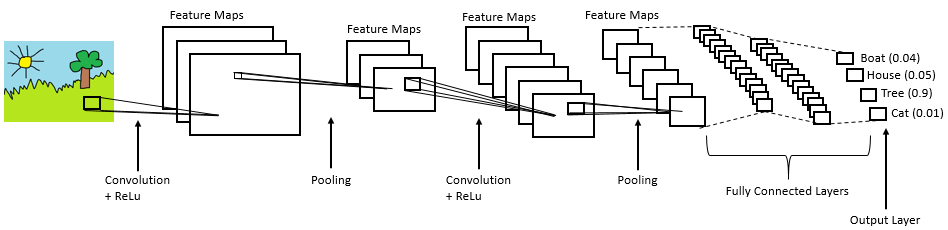
\includegraphics[width=.8\textwidth]{figures/cnn-illustration.png}
    \caption{Convolution on pixels in CNN}
    \label{cnn-illustration}
\end{figure}

\section{Fourier Transformation and Graph Convolution}

While graph data consists of node features and edge features, which are non-Euclidean Structure, the original convolution cannot apply on the data. In the work T. M. Kipf and M. Welling, the covolution operators are re-applied through different methods. The spectral graph theory provides fourier transformation and inverse fourier transformation, given discrete graph adjacency matrix $A$.

\begin{equation}
    \hat{f} = U^T f
    \label{discrete-fourier-transformation}
\end{equation}
    
\begin{equation}
    f = U \hat{f}
    \label{discrete-inverse-fourier-transformation}
\end{equation}

where $U$ is the eigenvector matrix in normalized symmetry graph Laplacian

\begin{equation}
    L = I_N - D^{-\frac{1}{2}}AD^{-\frac{1}{2}} = U\Lambda U^T
    \label{normalized-sysmetry-graph-laplacian}
\end{equation}

The character of fourier tranformation brings sound transformation between convolution operators and fourier operators in non-Euclidean field. 

\begin{equation}
    \begin{aligned}
        \mathcal{F} (h \ast f) & = \mathcal{F} (h) \cdot \mathcal{F} (f) \\
        (h \ast f)_G & = U\left(U^T(h)\odot U^T(f)\right) \\
    \end{aligned}
    \label{graph-convolution}
\end{equation}

where $\odot$ is the Hadamard Product. 

The calculation of graph convolution can be simplified throught the work of Hammond et al. on \textit{Wavelets on Graphs via Spectral Graph Theory}\cite{Hammond2009WaveletsOG}, gaining Equation \ref{approximated-graph-convolution}.

\begin{equation}
    (h \ast f)_{G'} = \sum _ {k=0} ^ K h' _ k T _ k (\tilde{L}) x
    \label{approximated-graph-convolution}
\end{equation}

where $T_k (x)$ denotes the $k$th Chebyshev polynomials, $h'$'s denote the Chebyshev coefficient vectors, $\tilde{L} = \frac{2}{\lambda_{max}}L - I_N$, $\lambda_{max}$ denotes the maximum eigenvalues of $L$, the normalized symmetry Laplacian. The detailed exploration should refer to work of Kipf et al.\cite{DBLP:journals/corr/KipfW16}

	
	% \chapter{Reproduction of GCN}

\section{Graph Convolution Layer and GCN model}

A neutral network based on graph convolution consists of layers of graph convolution and non-linear activation function. To reproduct the work of Kipf et al.\cite{DBLP:journals/corr/KipfW16}, a neutral network is modeled by the forward function in Equation \ref{forward-function-in-gcn}.

\begin{equation}
    Z = f(X, A) = \text{softmax} \left(\hat{A}\cdot \text{ReLU}\left(\hat{A}XW^{(0)}\right)W(1)\right)
    \label{forward-function-in-gcn}
\end{equation}

\section{Model Implement and Experiment}

The reproduced model is based on PyTorch package, which contains built-in neutral network model frameworks. The codes are attached in Appendix. 

To regain the training result in the work of Kipf et al\cite{DBLP:journals/corr/KipfW16}, the model implements the same hyperparameters, as shown in Table \ref{hyperparam-gcn}.

\medskip

\begin{table}[H]
    \centering
    \small
    \begin{tabular}{cccccc}
        \hline
        random seed & hidden units & dropout rate & learning rate & weight decay for L2 loss & epochs \\
        24 & 16 & 0.5 & 0.01 & 5e-4 & 200 \\
        \hline
    \end{tabular}
    \caption{Hyperparameters in GCN Reproduction}
    \label{hyperparam-gcn}
\end{table}

\section{Comparison and Result}

The training is carried out on \textbf{Cora} dataset\cite{Sen_Namata_Bilgic_Getoor_Galligher_Eliassi-Rad_2008} in both reproducable random split measures. The result performance is calculated on the basis on 20 trainings, which 

The original paper performance and comparison is shown in Table \ref{result-comparison}.

\begin{table}[H]
    \centering
    \small
    \begin{tabular}{lll}
        \hline
        model & Cora & Citeseer \\
        \hline
        ManiReg\cite{ManiReg} & 59.5 & 60.1 \\
        SemiEmb\cite{SemiEmb} & 59.0 & 59.6 \\
        LP\cite{LP} & 68.0 & 45.3 \\
        DeepWalk\cite{DeepWalk} & 67.2 & 43.2 \\
        ICA\cite{ICA} & 75.1 & 69.1 \\
        Planetoid*\cite{DBLP:journals/corr/YangCS16} & 75.7 & 64.7 \\
        GCN (paper) & 81.5 & 70.3 \\
        GCN (paper, rand splits) & 80.1$\pm$0.5 & 67.9$\pm$0.5 \\
        \hline
        GCN (reproduced) & 82.5 & 73.1 \\
        \hline
    \end{tabular}
    \caption{Comparison of GCN and Other Model Performance}
    \label{result-comparison}
\end{table}


The results of reproduction generally matches the original performance. The reproduction appears to have slightly higher accuracy rate, which can be caused by sample shuffling and difference in train-valid-test ratio. The reproduction is in all satisfactory.


	% \chapter{Further Study of GCN}

\section{Discussion of GCN}

Kipf et al.\cite{DBLP:journals/corr/KipfW16} modeled and trained the GCN on the whole graph set; whereas, the model reveals two shortcomings. The whole graph is stored in CPU/GPU in every epochs, which is computationally expensive and makes it hard to train on large-scale graph network. Meanwhile, mini-batch gradient descent cannot apply to the model, which should increase the stochasticity of the model. 

\section{Possible Improvements}

Improvements on mini-batch, which is in considerable complexity and beyond the mathematical ability of the author, are revealed by reviews on other researches.

\subsection{GCNSAGE}

\textit{Inductive Representation Learning on Large Graph} by Hamilton et al.\cite{DBLP:journals/corr/HamiltonYL17} presents GCNSAGE model, which utilizes low-dimensional node embeddings and feature sampling and aggregating. 

The implementation of each training iteration in GCNSAGE is in Table \ref{implementation-gcnsage}.

\begin{table}[H]
    \centering
    \noindent\rule{.7\textwidth}{1pt}

    \medskip

    \begin{varwidth}{.7\textwidth}
        \begin{itemize}
            \item Randomly select a minibatch $\upsilon_B\in \upsilon_L$ of nodes;
            \item Build a computation graph that only contains the activation $h_{\upsilon}^P(l)$ and $\bar{h}_{\upsilon}^{(l)}$ needed for the current minibatch;
            \item Get the predictions by forward propagation as $Z^{(l+1)} = \left(\hat{P}^{(l)}(H^{(l)} - \bar{H}^{(l)}) + P\bar{H}^{(l)}\right)W^{(l)}$;
            \item Get the gradients by backward propagation, and update the parameters by SGD;
            \item Update the historical activations;
        \end{itemize}
    \end{varwidth}
    
    \medskip
    
    \noindent\rule{.7\textwidth}{1pt}

    \caption{GCNSAGE Implementation}
    \label{implementation-gcnsage}
\end{table}

\subsection{FastGCN}

\textit{FastGCN: Fast Learning with Graph Convolutional Networks via Importance Sampling} by Chen et al.\cite{DBLP:journals/corr/abs-1801-10247}

\subsection{N-GCN}

\cite{DBLP:journals/corr/abs-1802-08888}

	
	\medskip

	%% If you want to use the bibliography feature, 
	%% 1. run latex on tex;
	%% 2. run 'biber outputs/[bcfname]' on prompt command line;
	%% 3. run latex on tex.

	\printbibliography

	\appendix{GCN Model Code}

	\inputminted{octave}{../model.py}
\end{document}
